% Created by tikzDevice version 0.12.3.1 on 2021-04-15 15:42:04
% !TEX encoding = UTF-8 Unicode
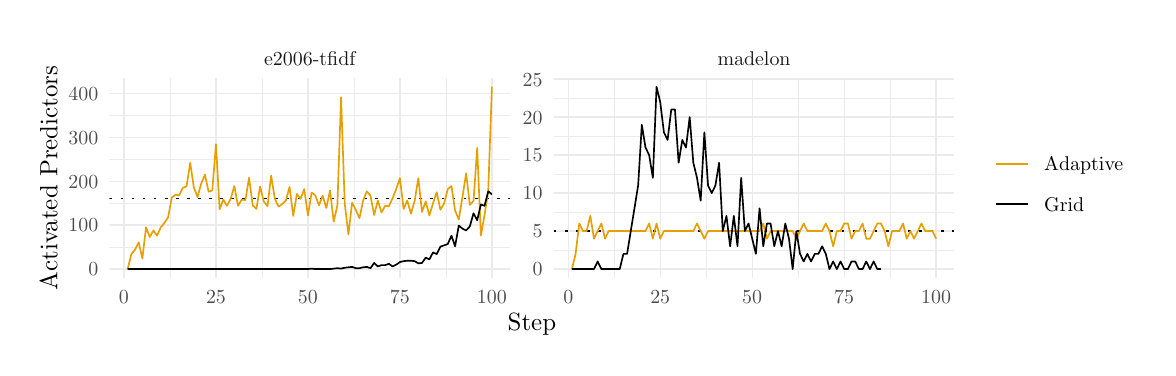
\begin{tikzpicture}[x=1pt,y=1pt]
\definecolor{fillColor}{RGB}{255,255,255}
\path[use as bounding box,fill=fillColor,fill opacity=0.00] (0,0) rectangle (404.71,115.63);
\begin{scope}
\path[clip] ( 29.55, 25.11) rectangle (174.33, 97.57);
\definecolor{drawColor}{gray}{0.92}

\path[draw=drawColor,line width= 0.2pt,line join=round] ( 29.55, 36.34) --
	(174.33, 36.34);

\path[draw=drawColor,line width= 0.2pt,line join=round] ( 29.55, 52.21) --
	(174.33, 52.21);

\path[draw=drawColor,line width= 0.2pt,line join=round] ( 29.55, 68.09) --
	(174.33, 68.09);

\path[draw=drawColor,line width= 0.2pt,line join=round] ( 29.55, 83.96) --
	(174.33, 83.96);

\path[draw=drawColor,line width= 0.2pt,line join=round] ( 51.42, 25.11) --
	( 51.42, 97.57);

\path[draw=drawColor,line width= 0.2pt,line join=round] ( 84.65, 25.11) --
	( 84.65, 97.57);

\path[draw=drawColor,line width= 0.2pt,line join=round] (117.89, 25.11) --
	(117.89, 97.57);

\path[draw=drawColor,line width= 0.2pt,line join=round] (151.13, 25.11) --
	(151.13, 97.57);

\path[draw=drawColor,line width= 0.5pt,line join=round] ( 29.55, 28.40) --
	(174.33, 28.40);

\path[draw=drawColor,line width= 0.5pt,line join=round] ( 29.55, 44.27) --
	(174.33, 44.27);

\path[draw=drawColor,line width= 0.5pt,line join=round] ( 29.55, 60.15) --
	(174.33, 60.15);

\path[draw=drawColor,line width= 0.5pt,line join=round] ( 29.55, 76.02) --
	(174.33, 76.02);

\path[draw=drawColor,line width= 0.5pt,line join=round] ( 29.55, 91.90) --
	(174.33, 91.90);

\path[draw=drawColor,line width= 0.5pt,line join=round] ( 34.80, 25.11) --
	( 34.80, 97.57);

\path[draw=drawColor,line width= 0.5pt,line join=round] ( 68.04, 25.11) --
	( 68.04, 97.57);

\path[draw=drawColor,line width= 0.5pt,line join=round] (101.27, 25.11) --
	(101.27, 97.57);

\path[draw=drawColor,line width= 0.5pt,line join=round] (134.51, 25.11) --
	(134.51, 97.57);

\path[draw=drawColor,line width= 0.5pt,line join=round] (167.75, 25.11) --
	(167.75, 97.57);
\definecolor{drawColor}{RGB}{0,0,0}

\path[draw=drawColor,line width= 0.6pt,dash pattern=on 1pt off 3pt ,line join=round] ( 29.55, 53.94) -- (174.33, 53.94);
\definecolor{drawColor}{RGB}{230,159,0}

\path[draw=drawColor,line width= 0.6pt,line join=round] ( 36.13, 28.40) --
	( 37.46, 33.80) --
	( 38.79, 35.39) --
	( 40.12, 38.08) --
	( 41.44, 32.21) --
	( 42.77, 43.48) --
	( 44.10, 39.99) --
	( 45.43, 42.37) --
	( 46.76, 40.47) --
	( 48.09, 43.48) --
	( 49.42, 45.07) --
	( 50.75, 47.13) --
	( 52.08, 54.28) --
	( 53.41, 55.23) --
	( 54.74, 55.07) --
	( 56.07, 57.77) --
	( 57.40, 58.24) --
	( 58.73, 66.82) --
	( 60.06, 57.77) --
	( 61.39, 54.43) --
	( 62.72, 59.36) --
	( 64.05, 62.53) --
	( 65.38, 56.34) --
	( 66.71, 56.82) --
	( 68.04, 73.48) --
	( 69.36, 49.99) --
	( 70.69, 53.48) --
	( 72.02, 51.26) --
	( 73.35, 53.80) --
	( 74.68, 58.40) --
	( 76.01, 51.26) --
	( 77.34, 53.48) --
	( 78.67, 53.32) --
	( 80.00, 61.42) --
	( 81.33, 51.42) --
	( 82.66, 50.15) --
	( 83.99, 58.24) --
	( 85.32, 52.85) --
	( 86.65, 51.10) --
	( 87.98, 62.21) --
	( 89.31, 53.80) --
	( 90.64, 50.94) --
	( 91.97, 51.89) --
	( 93.30, 53.16) --
	( 94.63, 58.09) --
	( 95.96, 47.61) --
	( 97.28, 55.55) --
	( 98.61, 53.80) --
	( 99.94, 57.29) --
	(101.27, 47.77) --
	(102.60, 56.02) --
	(103.93, 55.07) --
	(105.26, 51.42) --
	(106.59, 54.91) --
	(107.92, 50.47) --
	(109.25, 56.82) --
	(110.58, 45.54) --
	(111.91, 51.42) --
	(113.24, 90.47) --
	(114.57, 52.05) --
	(115.90, 40.94) --
	(117.23, 52.37) --
	(118.56, 49.83) --
	(119.89, 46.81) --
	(121.22, 53.16) --
	(122.55, 56.50) --
	(123.88, 54.91) --
	(125.20, 47.93) --
	(126.53, 53.16) --
	(127.86, 48.88) --
	(129.19, 51.26) --
	(130.52, 51.10) --
	(131.85, 53.96) --
	(133.18, 57.29) --
	(134.51, 61.26) --
	(135.84, 50.15) --
	(137.17, 53.16) --
	(138.50, 48.40) --
	(139.83, 53.01) --
	(141.16, 61.26) --
	(142.49, 49.04) --
	(143.82, 52.85) --
	(145.15, 47.77) --
	(146.48, 52.21) --
	(147.81, 56.18) --
	(149.14, 49.83) --
	(150.47, 52.05) --
	(151.80, 57.29) --
	(153.13, 58.40) --
	(154.45, 49.51) --
	(155.78, 46.34) --
	(157.11, 54.43) --
	(158.44, 63.01) --
	(159.77, 51.58) --
	(161.10, 53.01) --
	(162.43, 72.21) --
	(163.76, 40.47) --
	(165.09, 47.93) --
	(166.42, 56.66) --
	(167.75, 94.28);
\definecolor{drawColor}{RGB}{0,0,0}

\path[draw=drawColor,line width= 0.6pt,line join=round] ( 36.13, 28.40) --
	( 37.46, 28.40) --
	( 38.79, 28.40) --
	( 40.12, 28.40) --
	( 41.44, 28.40) --
	( 42.77, 28.40) --
	( 44.10, 28.40) --
	( 45.43, 28.40) --
	( 46.76, 28.40) --
	( 48.09, 28.40) --
	( 49.42, 28.40) --
	( 50.75, 28.40) --
	( 52.08, 28.40) --
	( 53.41, 28.40) --
	( 54.74, 28.40) --
	( 56.07, 28.40) --
	( 57.40, 28.40) --
	( 58.73, 28.40) --
	( 60.06, 28.40) --
	( 61.39, 28.40) --
	( 62.72, 28.40) --
	( 64.05, 28.40) --
	( 65.38, 28.40) --
	( 66.71, 28.40) --
	( 68.04, 28.40) --
	( 69.36, 28.40) --
	( 70.69, 28.40) --
	( 72.02, 28.40) --
	( 73.35, 28.40) --
	( 74.68, 28.40) --
	( 76.01, 28.40) --
	( 77.34, 28.40) --
	( 78.67, 28.40) --
	( 80.00, 28.40) --
	( 81.33, 28.40) --
	( 82.66, 28.40) --
	( 83.99, 28.40) --
	( 85.32, 28.40) --
	( 86.65, 28.40) --
	( 87.98, 28.40) --
	( 89.31, 28.40) --
	( 90.64, 28.40) --
	( 91.97, 28.40) --
	( 93.30, 28.40) --
	( 94.63, 28.40) --
	( 95.96, 28.40) --
	( 97.28, 28.40) --
	( 98.61, 28.40) --
	( 99.94, 28.40) --
	(101.27, 28.40) --
	(102.60, 28.56) --
	(103.93, 28.40) --
	(105.26, 28.40) --
	(106.59, 28.40) --
	(107.92, 28.40) --
	(109.25, 28.40) --
	(110.58, 28.56) --
	(111.91, 28.72) --
	(113.24, 28.56) --
	(114.57, 28.88) --
	(115.90, 29.04) --
	(117.23, 29.19) --
	(118.56, 28.72) --
	(119.89, 28.72) --
	(121.22, 29.04) --
	(122.55, 29.19) --
	(123.88, 28.72) --
	(125.20, 30.62) --
	(126.53, 29.35) --
	(127.86, 29.83) --
	(129.19, 29.83) --
	(130.52, 30.31) --
	(131.85, 29.35) --
	(133.18, 29.99) --
	(134.51, 30.94) --
	(135.84, 31.26) --
	(137.17, 31.42) --
	(138.50, 31.42) --
	(139.83, 31.26) --
	(141.16, 30.46) --
	(142.49, 30.62) --
	(143.82, 32.53) --
	(145.15, 31.89) --
	(146.48, 34.43) --
	(147.81, 33.80) --
	(149.14, 36.50) --
	(150.47, 36.97) --
	(151.80, 37.45) --
	(153.13, 40.47) --
	(154.45, 36.66) --
	(155.78, 44.12) --
	(157.11, 43.00) --
	(158.44, 42.37) --
	(159.77, 43.80) --
	(161.10, 48.56) --
	(162.43, 46.02) --
	(163.76, 51.74) --
	(165.09, 51.26) --
	(166.42, 56.50) --
	(167.75, 55.39);
\end{scope}
\begin{scope}
\path[clip] (190.08, 25.11) rectangle (334.86, 97.57);
\definecolor{drawColor}{gray}{0.92}

\path[draw=drawColor,line width= 0.2pt,line join=round] (190.08, 35.26) --
	(334.86, 35.26);

\path[draw=drawColor,line width= 0.2pt,line join=round] (190.08, 48.99) --
	(334.86, 48.99);

\path[draw=drawColor,line width= 0.2pt,line join=round] (190.08, 62.71) --
	(334.86, 62.71);

\path[draw=drawColor,line width= 0.2pt,line join=round] (190.08, 76.44) --
	(334.86, 76.44);

\path[draw=drawColor,line width= 0.2pt,line join=round] (190.08, 90.16) --
	(334.86, 90.16);

\path[draw=drawColor,line width= 0.2pt,line join=round] (211.95, 25.11) --
	(211.95, 97.57);

\path[draw=drawColor,line width= 0.2pt,line join=round] (245.19, 25.11) --
	(245.19, 97.57);

\path[draw=drawColor,line width= 0.2pt,line join=round] (278.43, 25.11) --
	(278.43, 97.57);

\path[draw=drawColor,line width= 0.2pt,line join=round] (311.66, 25.11) --
	(311.66, 97.57);

\path[draw=drawColor,line width= 0.5pt,line join=round] (190.08, 28.40) --
	(334.86, 28.40);

\path[draw=drawColor,line width= 0.5pt,line join=round] (190.08, 42.13) --
	(334.86, 42.13);

\path[draw=drawColor,line width= 0.5pt,line join=round] (190.08, 55.85) --
	(334.86, 55.85);

\path[draw=drawColor,line width= 0.5pt,line join=round] (190.08, 69.57) --
	(334.86, 69.57);

\path[draw=drawColor,line width= 0.5pt,line join=round] (190.08, 83.30) --
	(334.86, 83.30);

\path[draw=drawColor,line width= 0.5pt,line join=round] (190.08, 97.02) --
	(334.86, 97.02);

\path[draw=drawColor,line width= 0.5pt,line join=round] (195.33, 25.11) --
	(195.33, 97.57);

\path[draw=drawColor,line width= 0.5pt,line join=round] (228.57, 25.11) --
	(228.57, 97.57);

\path[draw=drawColor,line width= 0.5pt,line join=round] (261.81, 25.11) --
	(261.81, 97.57);

\path[draw=drawColor,line width= 0.5pt,line join=round] (295.05, 25.11) --
	(295.05, 97.57);

\path[draw=drawColor,line width= 0.5pt,line join=round] (328.28, 25.11) --
	(328.28, 97.57);
\definecolor{drawColor}{RGB}{0,0,0}

\path[draw=drawColor,line width= 0.6pt,dash pattern=on 1pt off 3pt ,line join=round] (190.08, 42.13) -- (334.86, 42.13);
\definecolor{drawColor}{RGB}{230,159,0}

\path[draw=drawColor,line width= 0.6pt,line join=round] (196.66, 28.40) --
	(197.99, 33.89) --
	(199.32, 44.87) --
	(200.65, 42.13) --
	(201.98, 42.13) --
	(203.31, 47.62) --
	(204.64, 39.38) --
	(205.97, 42.13) --
	(207.30, 44.87) --
	(208.63, 39.38) --
	(209.96, 42.13) --
	(211.29, 42.13) --
	(212.61, 42.13) --
	(213.94, 42.13) --
	(215.27, 42.13) --
	(216.60, 42.13) --
	(217.93, 42.13) --
	(219.26, 42.13) --
	(220.59, 42.13) --
	(221.92, 42.13) --
	(223.25, 42.13) --
	(224.58, 44.87) --
	(225.91, 39.38) --
	(227.24, 44.87) --
	(228.57, 39.38) --
	(229.90, 42.13) --
	(231.23, 42.13) --
	(232.56, 42.13) --
	(233.89, 42.13) --
	(235.22, 42.13) --
	(236.55, 42.13) --
	(237.88, 42.13) --
	(239.21, 42.13) --
	(240.53, 42.13) --
	(241.86, 44.87) --
	(243.19, 42.13) --
	(244.52, 39.38) --
	(245.85, 42.13) --
	(247.18, 42.13) --
	(248.51, 42.13) --
	(249.84, 42.13) --
	(251.17, 42.13) --
	(252.50, 42.13) --
	(253.83, 42.13) --
	(255.16, 42.13) --
	(256.49, 42.13) --
	(257.82, 42.13) --
	(259.15, 42.13) --
	(260.48, 42.13) --
	(261.81, 42.13) --
	(263.14, 42.13) --
	(264.47, 42.13) --
	(265.80, 44.87) --
	(267.13, 39.38) --
	(268.45, 42.13) --
	(269.78, 42.13) --
	(271.11, 42.13) --
	(272.44, 42.13) --
	(273.77, 42.13) --
	(275.10, 42.13) --
	(276.43, 42.13) --
	(277.76, 39.38) --
	(279.09, 42.13) --
	(280.42, 44.87) --
	(281.75, 42.13) --
	(283.08, 42.13) --
	(284.41, 42.13) --
	(285.74, 42.13) --
	(287.07, 42.13) --
	(288.40, 44.87) --
	(289.73, 42.13) --
	(291.06, 36.64) --
	(292.39, 42.13) --
	(293.72, 42.13) --
	(295.05, 44.87) --
	(296.38, 44.87) --
	(297.70, 39.38) --
	(299.03, 42.13) --
	(300.36, 42.13) --
	(301.69, 44.87) --
	(303.02, 39.38) --
	(304.35, 39.38) --
	(305.68, 42.13) --
	(307.01, 44.87) --
	(308.34, 44.87) --
	(309.67, 42.13) --
	(311.00, 36.64) --
	(312.33, 42.13) --
	(313.66, 42.13) --
	(314.99, 42.13) --
	(316.32, 44.87) --
	(317.65, 39.38) --
	(318.98, 42.13) --
	(320.31, 39.38) --
	(321.64, 42.13) --
	(322.97, 44.87) --
	(324.30, 42.13) --
	(325.62, 42.13) --
	(326.95, 42.13) --
	(328.28, 39.38);
\definecolor{drawColor}{RGB}{0,0,0}

\path[draw=drawColor,line width= 0.6pt,line join=round] (196.66, 28.40) --
	(197.99, 28.40) --
	(199.32, 28.40) --
	(200.65, 28.40) --
	(201.98, 28.40) --
	(203.31, 28.40) --
	(204.64, 28.40) --
	(205.97, 31.15) --
	(207.30, 28.40) --
	(208.63, 28.40) --
	(209.96, 28.40) --
	(211.29, 28.40) --
	(212.61, 28.40) --
	(213.94, 28.40) --
	(215.27, 33.89) --
	(216.60, 33.89) --
	(217.93, 42.13) --
	(219.26, 50.36) --
	(220.59, 58.60) --
	(221.92, 80.55) --
	(223.25, 72.32) --
	(224.58, 69.57) --
	(225.91, 61.34) --
	(227.24, 94.28) --
	(228.57, 88.79) --
	(229.90, 77.81) --
	(231.23, 75.06) --
	(232.56, 86.04) --
	(233.89, 86.04) --
	(235.22, 66.83) --
	(236.55, 75.06) --
	(237.88, 72.32) --
	(239.21, 83.30) --
	(240.53, 66.83) --
	(241.86, 61.34) --
	(243.19, 53.11) --
	(244.52, 77.81) --
	(245.85, 58.60) --
	(247.18, 55.85) --
	(248.51, 58.60) --
	(249.84, 66.83) --
	(251.17, 42.13) --
	(252.50, 47.62) --
	(253.83, 36.64) --
	(255.16, 47.62) --
	(256.49, 36.64) --
	(257.82, 61.34) --
	(259.15, 42.13) --
	(260.48, 44.87) --
	(261.81, 39.38) --
	(263.14, 33.89) --
	(264.47, 50.36) --
	(265.80, 36.64) --
	(267.13, 44.87) --
	(268.45, 44.87) --
	(269.78, 36.64) --
	(271.11, 42.13) --
	(272.44, 36.64) --
	(273.77, 44.87) --
	(275.10, 39.38) --
	(276.43, 28.40) --
	(277.76, 42.13) --
	(279.09, 33.89) --
	(280.42, 31.15) --
	(281.75, 33.89) --
	(283.08, 31.15) --
	(284.41, 33.89) --
	(285.74, 33.89) --
	(287.07, 36.64) --
	(288.40, 33.89) --
	(289.73, 28.40) --
	(291.06, 31.15) --
	(292.39, 28.40) --
	(293.72, 31.15) --
	(295.05, 28.40) --
	(296.38, 28.40) --
	(297.70, 31.15) --
	(299.03, 31.15) --
	(300.36, 28.40) --
	(301.69, 28.40) --
	(303.02, 31.15) --
	(304.35, 28.40) --
	(305.68, 31.15) --
	(307.01, 28.40) --
	(308.34, 28.40);
\end{scope}
\begin{scope}
\path[clip] ( 29.55, 97.57) rectangle (174.33,111.13);
\definecolor{drawColor}{gray}{0.10}

\node[text=drawColor,anchor=base,inner sep=0pt, outer sep=0pt, scale=  0.72] at (101.94,101.87) {e2006-tfidf};
\end{scope}
\begin{scope}
\path[clip] (190.08, 97.57) rectangle (334.86,111.13);
\definecolor{drawColor}{gray}{0.10}

\node[text=drawColor,anchor=base,inner sep=0pt, outer sep=0pt, scale=  0.72] at (262.47,101.87) {madelon};
\end{scope}
\begin{scope}
\path[clip] (  0.00,  0.00) rectangle (404.71,115.63);
\definecolor{drawColor}{gray}{0.30}

\node[text=drawColor,anchor=base,inner sep=0pt, outer sep=0pt, scale=  0.72] at ( 34.80, 16.10) {0};

\node[text=drawColor,anchor=base,inner sep=0pt, outer sep=0pt, scale=  0.72] at ( 68.04, 16.10) {25};

\node[text=drawColor,anchor=base,inner sep=0pt, outer sep=0pt, scale=  0.72] at (101.27, 16.10) {50};

\node[text=drawColor,anchor=base,inner sep=0pt, outer sep=0pt, scale=  0.72] at (134.51, 16.10) {75};

\node[text=drawColor,anchor=base,inner sep=0pt, outer sep=0pt, scale=  0.72] at (167.75, 16.10) {100};
\end{scope}
\begin{scope}
\path[clip] (  0.00,  0.00) rectangle (404.71,115.63);
\definecolor{drawColor}{gray}{0.30}

\node[text=drawColor,anchor=base,inner sep=0pt, outer sep=0pt, scale=  0.72] at (195.33, 16.10) {0};

\node[text=drawColor,anchor=base,inner sep=0pt, outer sep=0pt, scale=  0.72] at (228.57, 16.10) {25};

\node[text=drawColor,anchor=base,inner sep=0pt, outer sep=0pt, scale=  0.72] at (261.81, 16.10) {50};

\node[text=drawColor,anchor=base,inner sep=0pt, outer sep=0pt, scale=  0.72] at (295.05, 16.10) {75};

\node[text=drawColor,anchor=base,inner sep=0pt, outer sep=0pt, scale=  0.72] at (328.28, 16.10) {100};
\end{scope}
\begin{scope}
\path[clip] (  0.00,  0.00) rectangle (404.71,115.63);
\definecolor{drawColor}{gray}{0.30}

\node[text=drawColor,anchor=base east,inner sep=0pt, outer sep=0pt, scale=  0.72] at (186.03, 25.92) {0};

\node[text=drawColor,anchor=base east,inner sep=0pt, outer sep=0pt, scale=  0.72] at (186.03, 39.65) {5};

\node[text=drawColor,anchor=base east,inner sep=0pt, outer sep=0pt, scale=  0.72] at (186.03, 53.37) {10};

\node[text=drawColor,anchor=base east,inner sep=0pt, outer sep=0pt, scale=  0.72] at (186.03, 67.10) {15};

\node[text=drawColor,anchor=base east,inner sep=0pt, outer sep=0pt, scale=  0.72] at (186.03, 80.82) {20};

\node[text=drawColor,anchor=base east,inner sep=0pt, outer sep=0pt, scale=  0.72] at (186.03, 94.55) {25};
\end{scope}
\begin{scope}
\path[clip] (  0.00,  0.00) rectangle (404.71,115.63);
\definecolor{drawColor}{gray}{0.30}

\node[text=drawColor,anchor=base east,inner sep=0pt, outer sep=0pt, scale=  0.72] at ( 25.50, 25.92) {0};

\node[text=drawColor,anchor=base east,inner sep=0pt, outer sep=0pt, scale=  0.72] at ( 25.50, 41.80) {100};

\node[text=drawColor,anchor=base east,inner sep=0pt, outer sep=0pt, scale=  0.72] at ( 25.50, 57.67) {200};

\node[text=drawColor,anchor=base east,inner sep=0pt, outer sep=0pt, scale=  0.72] at ( 25.50, 73.54) {300};

\node[text=drawColor,anchor=base east,inner sep=0pt, outer sep=0pt, scale=  0.72] at ( 25.50, 89.42) {400};
\end{scope}
\begin{scope}
\path[clip] (  0.00,  0.00) rectangle (404.71,115.63);
\definecolor{drawColor}{RGB}{0,0,0}

\node[text=drawColor,anchor=base,inner sep=0pt, outer sep=0pt, scale=  0.90] at (182.21,  6.25) {Step};
\end{scope}
\begin{scope}
\path[clip] (  0.00,  0.00) rectangle (404.71,115.63);
\definecolor{drawColor}{RGB}{0,0,0}

\node[text=drawColor,rotate= 90.00,anchor=base,inner sep=0pt, outer sep=0pt, scale=  0.90] at ( 10.70, 61.34) {Activated Predictors};
\end{scope}
\begin{scope}
\path[clip] (  0.00,  0.00) rectangle (404.71,115.63);
\definecolor{drawColor}{RGB}{230,159,0}

\path[draw=drawColor,line width= 0.6pt,line join=round] (349.81, 66.32) -- (361.37, 66.32);
\end{scope}
\begin{scope}
\path[clip] (  0.00,  0.00) rectangle (404.71,115.63);
\definecolor{drawColor}{RGB}{0,0,0}

\path[draw=drawColor,line width= 0.6pt,line join=round] (349.81, 51.86) -- (361.37, 51.86);
\end{scope}
\begin{scope}
\path[clip] (  0.00,  0.00) rectangle (404.71,115.63);
\definecolor{drawColor}{RGB}{0,0,0}

\node[text=drawColor,anchor=base west,inner sep=0pt, outer sep=0pt, scale=  0.72] at (367.32, 63.84) {Adaptive};
\end{scope}
\begin{scope}
\path[clip] (  0.00,  0.00) rectangle (404.71,115.63);
\definecolor{drawColor}{RGB}{0,0,0}

\node[text=drawColor,anchor=base west,inner sep=0pt, outer sep=0pt, scale=  0.72] at (367.32, 49.38) {Grid};
\end{scope}
\end{tikzpicture}
